\chapter{Graphical Approach To Analyzing Transmission Line Problems Using Smith Chart}\label{lec:lec15}
We are going to solve few problems on transmission line mainly using smith chart. Measurement of an unknown impedance at high frequencies are carried out by studying the standing wave ratio and the location of the maxima and minima, of the standing wave pattern by using a\footnote{Slotted lines are used for microwave measurements and consist of a movable probe inserted into a slot in a transmission line. They are used in conjunction with a microwave power source and usually, in keeping with their low-cost application, a low cost Schottky diode detector and VSWR meter rather than an expensive microwave power meter.} slotted transmission line since measurement of phase is unreliable at high frequencies.

\begin{example}
\begin{figure}[h]
\centering
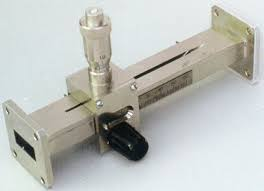
\includegraphics[width=1\linewidth]{./graphics/fig3}
\label{fig:fig3}
\caption{slotted transmission line.}
\end{figure}

We look at the example at figure~\ref{fig:fig3}, we have a transmission line to which an unknown impedance $Z_L$ is connected.By using what we call a slotted transmission line, we measure the standing wave pattern on the transmission line. With $\dfrac{\lambda}{2}=30cm$ where $\lambda=60cm.$
$$\phi=2\beta L$$ 
and 
\begin{dmath*}
\beta=\dfrac{2\pi}{\lambda}
\end{dmath*}
\begin{dmath*}
\phi=2\cdot\dfrac{2\pi}{\lambda} L
\end{dmath*}
$$\phi=2\cdot\dfrac{360}{60}\cdot27$$
$$\phi=324^{o}$$
\begin{figure}[h]
\centering
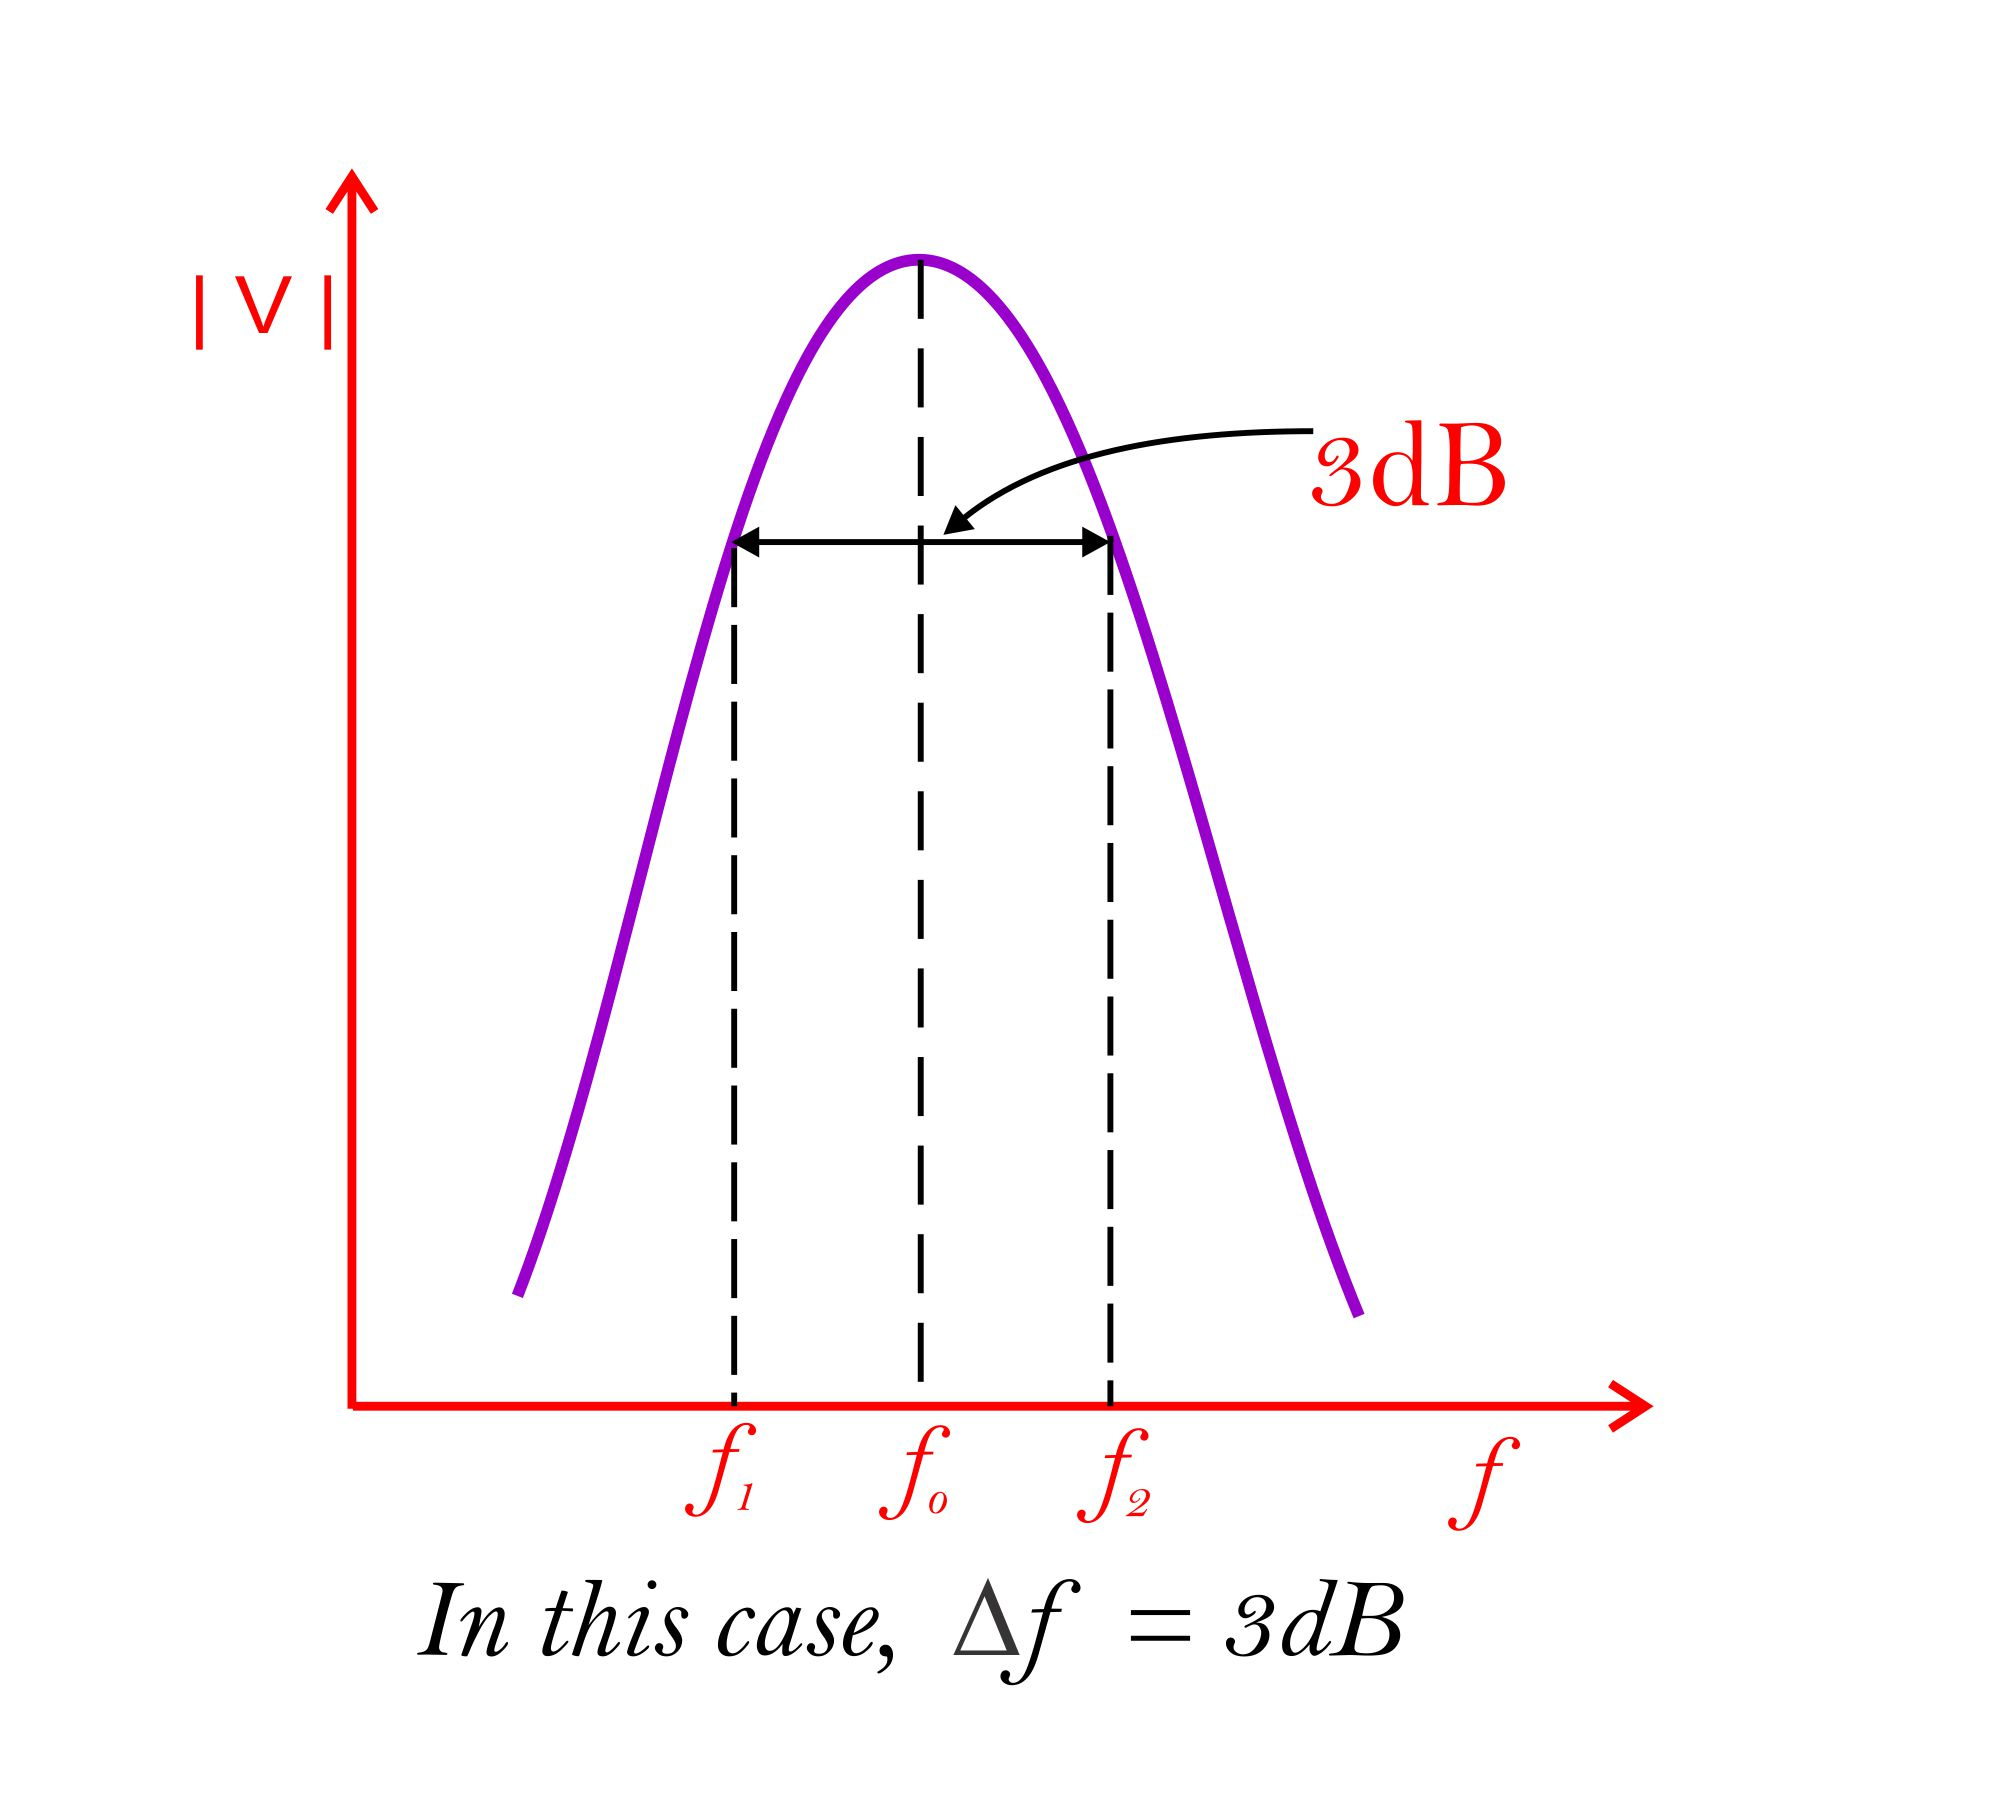
\includegraphics[width=1\linewidth]{./graphics/fig2}
\caption{Measurement Of Impedance}
\end{figure}
\begin{figure}[h]
\centering
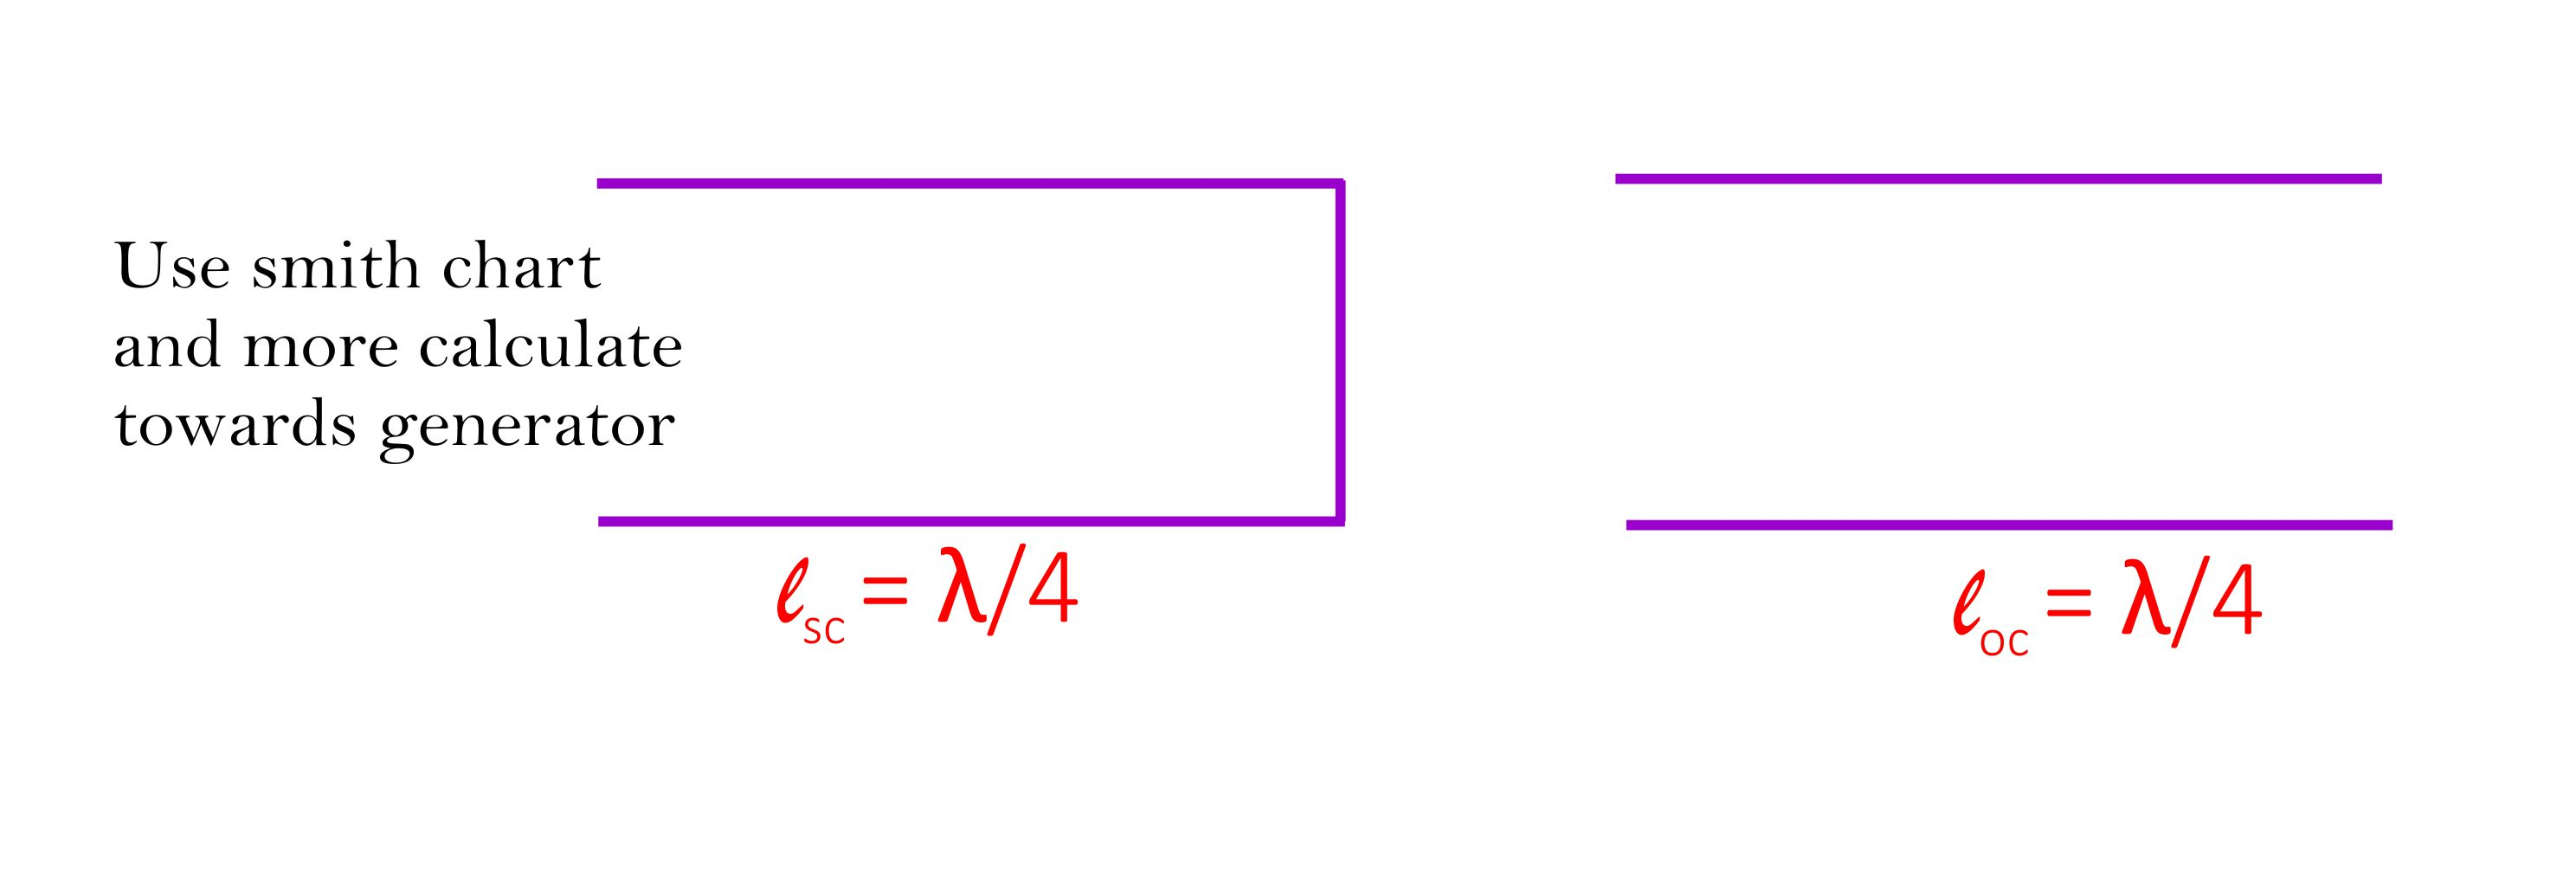
\includegraphics[width=1\linewidth]{./graphics/fig1}
\caption{Measurement Of Impedance}
\end{figure}

We measure the variation of voltage as a function of length $ l $ on the transmission line. With $V_{max}=15V,V_{min}=5V$
\begin{equation*}
\rho=\frac{V_{max}}{V_{min}}=\frac{15}{5}=3
\end{equation*}
With all these information,we go to the smith chart to calculate the unknown impedance.It is clear from here that moving a distance of $27cm$ from the load towards the generator. i.e clockwise  movement on the smith chart will correspond to $324^o$,
\begin{figure}[h]
\centering
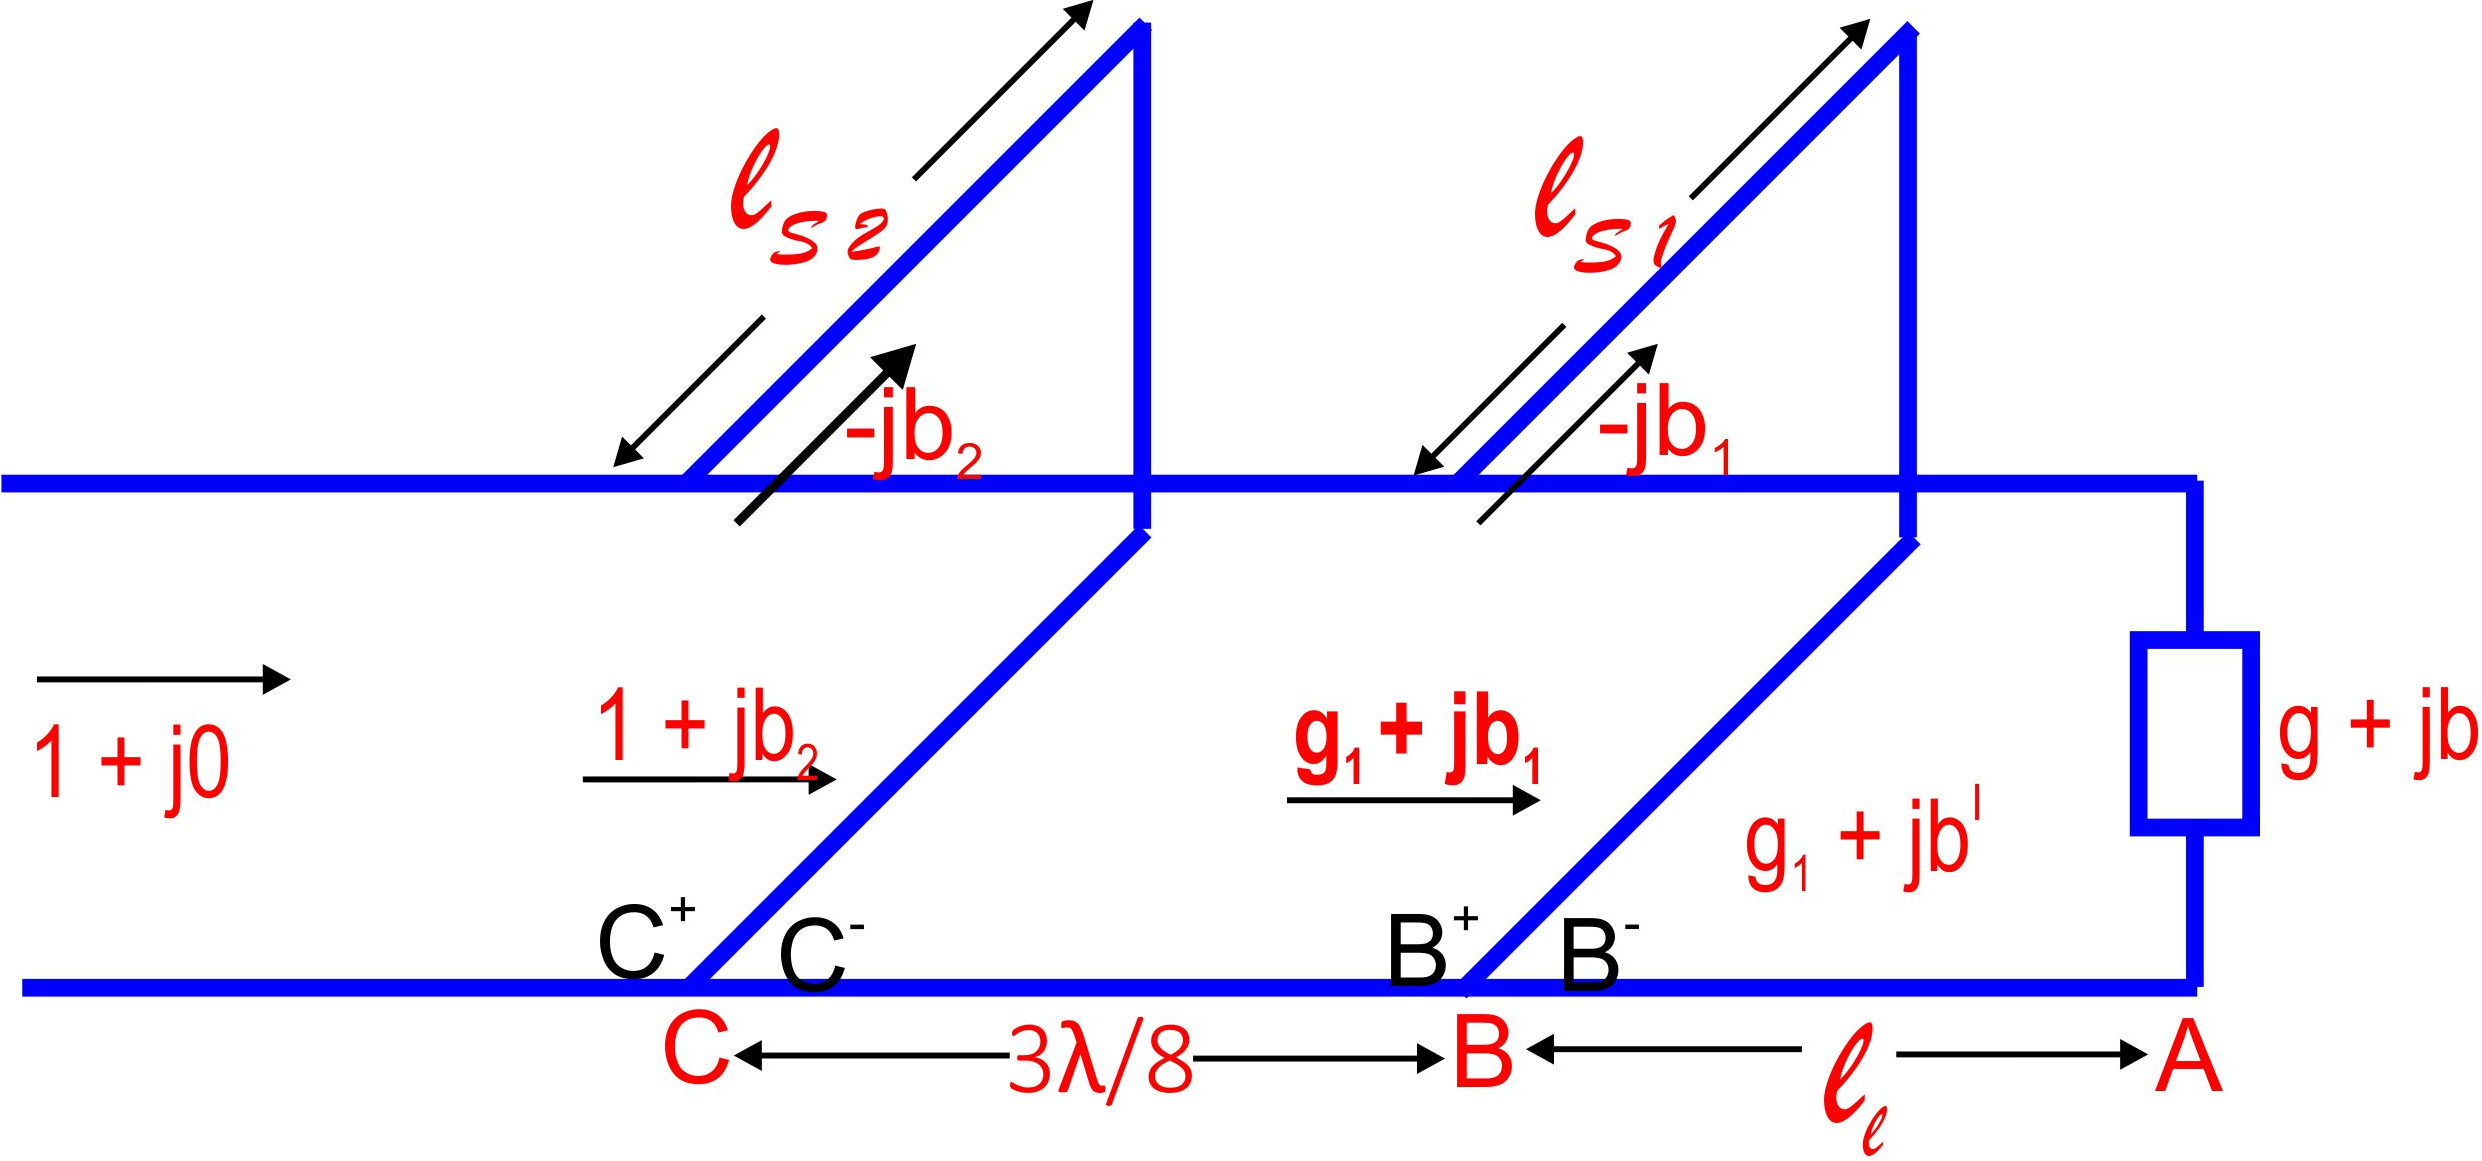
\includegraphics[width=1\linewidth]{./graphics/fig12}
\caption{Measurement of unknown impedance using smith chart}
\end{figure}

We should arrive at the maxima point on the impedance smith chart,which is the right hand intercept of the constant VSWR circle on the positive real axis. From origin we draw circle with \ radius= $\rho =3$,It touch the real axis at $V_{min}\ and\ V_{max}$. Where the angle cuts the VSWR=3 circle is the unknown impedance $\overline{Z}_L$ from the smith chart.In the smith chart $\overline{Z}_L=1.15-j1.23$. If the characteristics impedance of the line is $50\Omega$, then $Z_{L}= (\overline{Z}_L\times Z_o)=50(1.15-j1.23)= 57.5-j61.5 \Omega$. So unknown impedance can be measured very easily with a smith chart without doing much complex calculation.
\end{example}

\begin{example}
\subsection*{Problem using quarter wave transformer.}
A load impedance $Z_{L}=75-j35\Omega$ is to be matched to $50\Omega$ using quarter wave transformer.Design the matching set up. 
\begin{figure}[h]
\centering
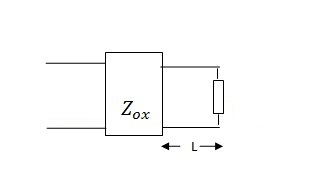
\includegraphics[width=1\linewidth]{./graphics/fighalfwave}
\caption{Load impedance matching}
\end{figure}

\subsection*{Solution}
We recall that the quarter wave transformer can match two resistive impedances if the characteristics impedance is real. However the impedance given to us here is complex,so we use a section of a transmission line to first convert the impedance to a real value, from that point onward a quarter wave transformer can then be used for the matching.\\
The length of the quarter wave  transformer is $\dfrac{\lambda}{4}$ at XX, 75-j35 should be real.
\begin{figure}[h]
\centering
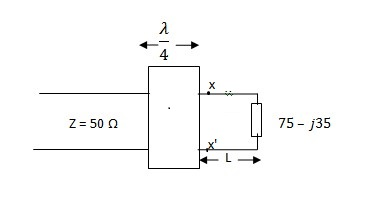
\includegraphics[width=1\linewidth]{./graphics/image}
\caption{Quarter wave transformer}
\end{figure}

On the smith chart we draw the VSWR circle for $Z_{L} =75-j35\Omega$ and move around it towards generator i.e in clockwise direction till we are in the real axis which gives $R_{min}\ and\ R_{max}\ or\ V_{min}\ and\ V_{max}$ respectively. \\
At  $ \overline{Z}_L=1.5-j0.7$ , marked on the smith chart using OX as radius, we draw constant VSWR circle that intercept the real axis at P and Q, if we move XP we get a real impedance corresponding to $R_{min}$ and if we move XPQ we get another real Impedance Corresponding to $R_{max}$. So we have two possibilities for either XP or XPQ.
\begin{figure}[h]
\centering
\includegraphics[width=1\linewidth]{./graphics/tosin}
\caption{Quarter wave transformer solution on smith chart}
\end{figure}

$$XP=0.5\lambda-0.306\lambda=0.194 \lambda=L_1$$
$\overline{R}_{min} =0.5\Omega$ on the smith chart,
\begin{dmath*}
R_{min}=Z_{o} \times \overline{R}_{min}=50\times0.5=25\Omega
\end{dmath*}
$$XPQ=0.194\lambda+0.25\lambda=0.444\lambda=L_2$$
$$\overline{R}_{max}=2\Omega$$
$$R_{max}=Z_{o} \times \overline{R}_{max}=50\times2=100\Omega$$
Hence $l=L_1=0.194\lambda \ or \ L_2=0.444\lambda$ which is the distance to be moved to change $Z_{L}$ to a real value of the quarter wavelength transformer. 
The outward circle of the smith chart is calibrated in $\lambda$,so you can take the angle subtended by the movement and do a direct conversion to $\lambda$, $\lambda$\ at X is 0.306 moving to 0.5 is a difference of 0.194$\lambda$\footnote{$L_1=0.5\lambda - 0.306\lambda=0.194\lambda$}
The top half is $0.25\lambda$, added to the 0.194$\lambda$ calculated initially brings us to 0.444$\lambda$ \footnote{$L_2=0.25\lambda+0.194\lambda=0.444\lambda$}
for $R_{max}$. Going back to the problem we have that for $L_1=0.194\lambda, R_{min}=25\varOmega$ 
\begin{equation*}
Z_{ox} \footnote{$Z_{ox}$is the geometric mean of the two impedances to be matched.}=\sqrt{Z_o\times R}=\sqrt{50\times25}=35.35\varOmega
\end{equation*}
For $$L_2=0.444\lambda, R_{max}=100\varOmega$$ 
\begin{dmath*}
Z_{ox}$ =$\sqrt{Z_o\times R}=\sqrt{50\times100}=70.7\varOmega
\end{dmath*}

Here we see how to match a complex impedance to a real impedance by using section of the transmission line and the quarter wavelength transformer. The quarter wavelength transformer can match only impedance which is real. That is why we introduce a section of transmission line before the quarter wavelength transformer to help convert our complex load impedance to real impedance.
\end{example}

\begin{example}
\subsection*{Problem on single stub matching.}
The main transmission line and the auxiliary line has $Z_o=50\varOmega$. Calculate $L_s\ and\ L_1$ using smith chart.
\begin{figure}[h]
\centering
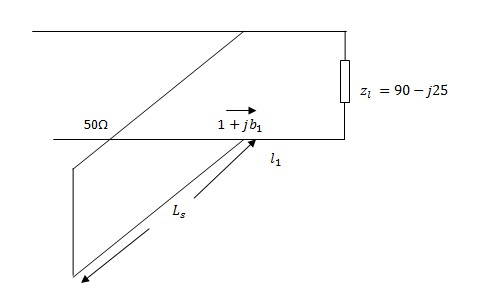
\includegraphics[width=1\linewidth]{./graphics/figw}
\caption{single stub matching}
\end{figure}
\subsection*{Solution}
We normalize $Z_L=90-j25$ to get 
$\overline{Z}_L=1.8-j0.5$. since stub and $Z_L$ are in parallel,
we convert $\overline{Z}_L$ to its admittance value. $\overline{Y}_{L}$
should be transformed from 
$\overline{Y}_{L}$=$g+jb$ to $1+jb_1$ hence it lies  on  the circle of constant conductance $g=1$. With OP we draw circle of constant VSWR with OP as radius. We get the point where this VSWR circle intercept the g=1 circle at moving clockwise(towards generator )from Q to M. the distance QM correspond to $L_1, L_1=0.152\lambda-0.032\lambda=0.12\lambda$.

Mirror M on the VSWR circle to get $1-jb1$. On the constant suceptance curve of $?jb$, find where it intercept the circle at $g=0 \ and \ ?jb_1$. This is the outermost circle. $R$ represent pure susceptance value of $jb_1$. 
\begin{figure}[h]
\centering
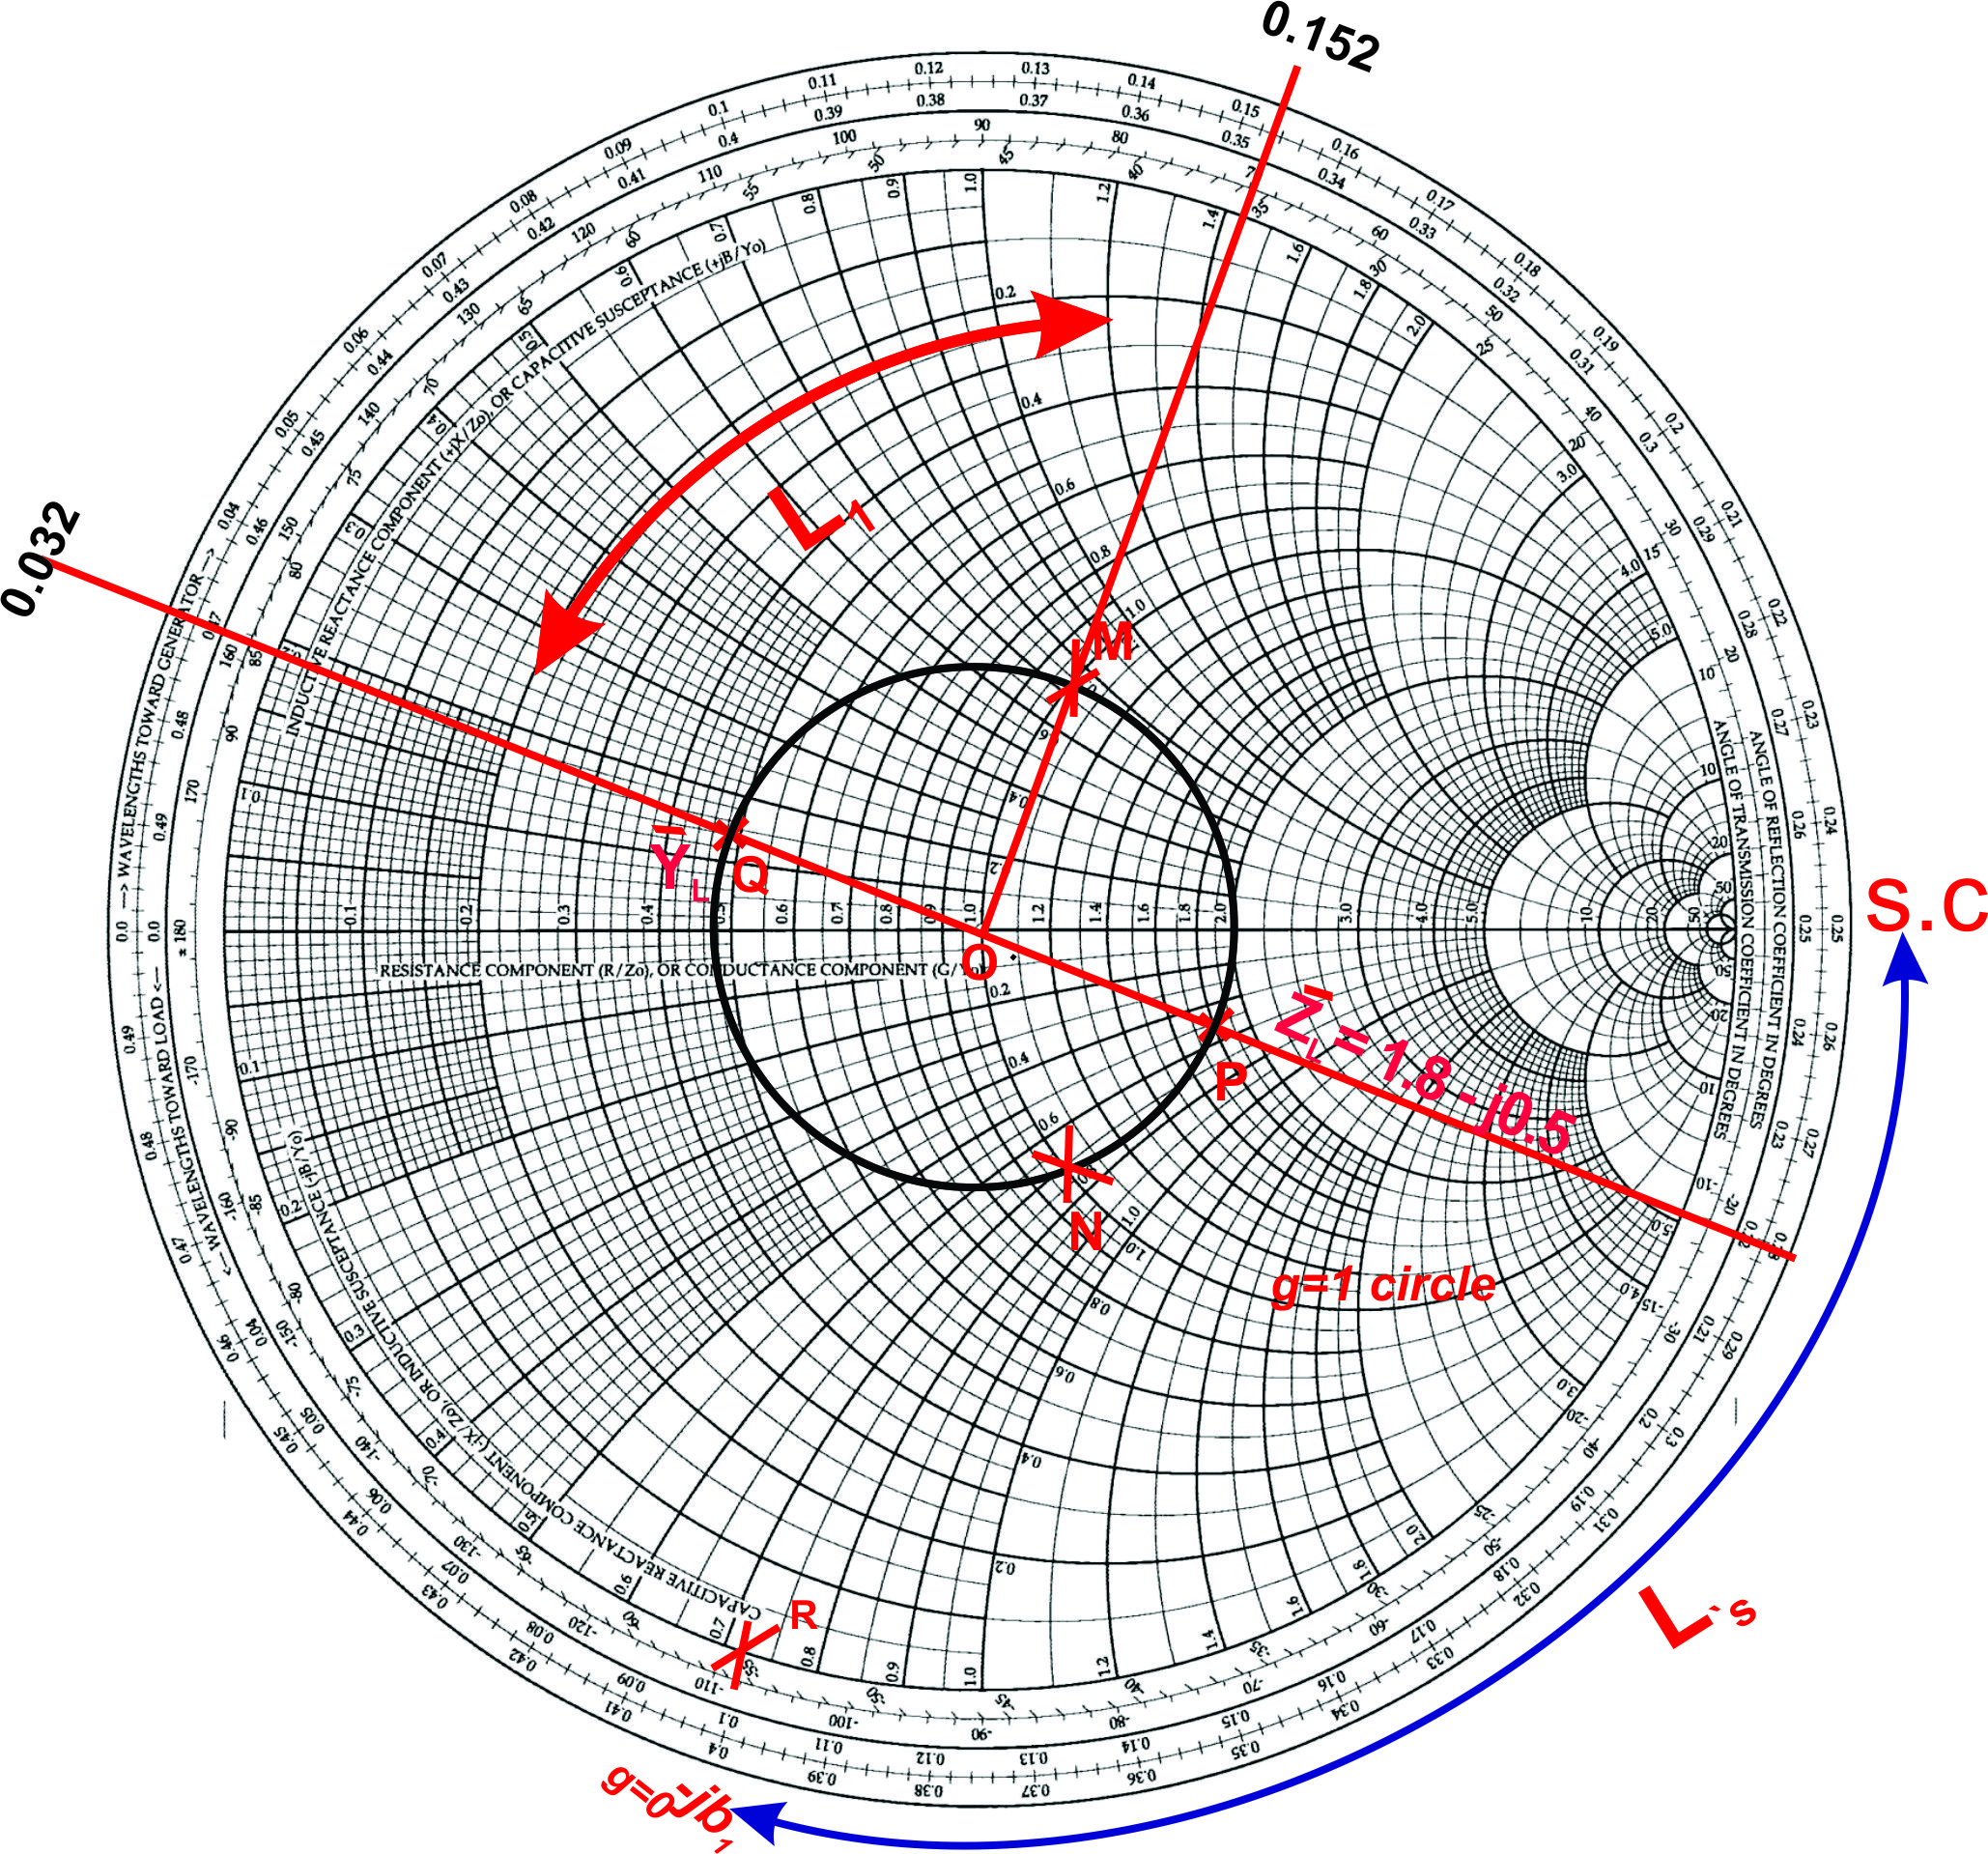
\includegraphics[width=1\linewidth]{./graphics/fig14}
\caption{single stub matching on a smith chart}
\end{figure}

Hence we have to move from SC \footnote{S.C- short circuit.} of the stub towards the generator to see this Susceptance.The distance $L_s$ is the movement from SC to -jb1 towards the generator and that distance represents the length of the stub.For admittance on smith chart right most side is the SC part and the leftmost  part is the open circuit part.This is  opposite to the convention in the impedance smith chart.\\
At SC $l_{s.c}=0.25\lambda$ moving towards the generator.At R, $l=0.402\lambda$,the distance $l_s=0.402-0.25=0.152\lambda$. Now we know the length of the stub and location of the stub as well.These are some of the problems which can be solved easily with the help of the smith chart.Using an analytic approach for the same  process is an extremely tedious task.This example clearly demonstrate the use of a smith  chart for solving complex transmission line problems.
\end{example}

\section{Characteristics impedance for common transmission line}
Let us talk about the final aspect of transmission line which is the characteristics impedance of common transmission line which we see in practice.At the beginning of our study, we saw various kinds of transmission line such as coaxial line,Parallel wire, Micro-strip structure e.t.c in practice one would need to calculate the characteristics impedance of the line.Let us see the formulas used for calculating the characteristics impedance of the various transmission line. The most commonly used transmission line is the Coaxial line commonly used for connection between  electric equipments.

\subsection{Coaxial line}
The coaxial cable has an inner diameter $d$ outer  diameter $D$ and dielectric constant $\epsilon_r$ for the medium separating the outer and inner conductor. Teflon is mostly used to separate d from D as the dielectric material is from 2 to 4 in value.
\begin{figure}[h]
\centering
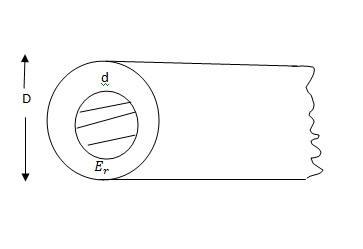
\includegraphics[width=1\linewidth]{./graphics/coaxialcable1}
\caption{coaxial line}
\end{figure}
\begin{figure}[h]
\centering
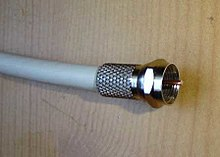
\includegraphics[scale=0.8]{./graphics/coaxialcable}
\caption{Typical image of a coaxial line}
\end{figure}

For this structure the characteristics impedance $Z_o$ is.
\begin{equation*}
Z_o=\dfrac{138}{\sqrt{\epsilon_r}}\log(\dfrac{D}{d})
\end{equation*}

The characteristics impedance of a coaxial line depends on the ratio of outer to inner diameters, and the dielectric constant separating the inner and the outer diameters.
We take some typical values just to get a feel of what kind of parameters are required to realize certain characteristics impedance, say $\epsilon_r$=4, $$Z_o=\dfrac{138}{\sqrt{4}}log(\dfrac{D}{d})$$ $$Z_o=69\log(\dfrac{D}{d})$$ $$\dfrac{D}{d}=10^{(\dfrac{Z_o}{69})}$$
What we see from this relationship is that the ratio of $\dfrac{D}{d}$  increases very rapidly as the characteristic of impedance $Z_o$ increases. When $Z_o=69\varOmega$ , $\dfrac{D}{d}=10$ or  $D=10d$ when $Z_o = 138$
\begin{dmath*}
\dfrac{D}{d}=10^{(\dfrac{138}{69})}=10^{2}=100
\end{dmath*}
therefore $D=100d$.

So the size of the outer conductor compared to the inner conductor increases very rapidly as the characteristics impedance of the line increases. What it means is that, the coaxial structure is more suited for realizing low characteristics impedances.That is the reason why typically the lines which are used as coaxial lines ,their characteristics impedance lies around $50\Omega$ to $75\Omega$. If we say lets realize a characteristics impedance of 200 or 300 ohms with same structure, $\dfrac{D}{d}=10^{(\dfrac{300}{69})}$=$22275.4$,this is an outrageous value of D/d and this size will be physically prohibitive.We will not be able to realize this structure. Hence, the coaxial structure is intrinsically more suited for realizing low characteristics impedances of order $50\Omega or 75\Omega$. Typically the cables are standardized for $50\Omega$, however when we go for antenna application we get a cable that has $75\Omega$ characteristics impedance  and the reason is that the antenna most used in practice i.e the half wave dipole has input impedance very close to $75\Omega$ as we shall see later,so just from the compatibility point of view of the impedances, whenever we use the cables for the antenna, we use the cable which is having a characteristics impedance of $75\Omega$. However for most of other application of high frequency equipment the impedance has been almost standardized to $50\Omega$

\subsection{Parallel wire transmission line(Balanced)} 
As the name suggest it has two conductors which are parallel with conductor diameter d and separation between the two conductors as D. Normally this arrangement is used in the air, so that the dielectric material separating them is air with\ $\epsilon_r=1$. However  there are some applications where they are insulated from each with another material not air and encapsulated in a material casing, in this case $\epsilon_r\neq1$. You would see this structure in something like overhead power line,you also see this structure when you make use of flat ribbon cable to connect yagi antenna to a TV. The flat ribbon cable which connects from the yagi antenna to a TV is essentially a parallel wire structure.
\begin{figure}[h]
\centering
\includegraphics[width=1\linewidth]{./graphics/FIG8}
\caption{parallel wire transmission line}
\end{figure}


In that case there is no air medium,you are having plastic encapsulation on that shown below with  $\epsilon_r\neq1$,the characteristics impedance of this structure is given by the formula 
\begin{equation*}
Z_o=\dfrac{276}{\sqrt{\epsilon_r}}\log(\dfrac{2D}{d})
\end{equation*}

$\epsilon_r$=1 when air is the dielectric separation so that $Z_o$=$276\log(\dfrac{2D}{d})$ we can only make D as small as possible to vary $Z_o$ . if $D\approx d$ i.e almost close to each other then $Z_o$=$276\log(\dfrac{2d}{d})$=$276\log(2)$=$82.8\Omega$. So minimum realizable value of D is when D = d, and at that point $Z_{min}=82.2\Omega$. With $\dfrac{D}{d}=5$ say $Z_o=276\log(2\times5)=276\log(10)=276\Omega$ As you can see for this structure realizing low impedance is more difficult, we can't realize impedance less than $82.8\Omega$. However we can realize high impedance easily. Since we are talking about two conductor which are parallel, separating them to vary $D$ is very easy.

This kind of transmission line intrinsically is used for realizing high characteristics impedance,these lines are also used in telephone lines,all the telephone lines which you see in towers are in the form of parallel wire lines,so generally the parallel wire transmission line are used in that application where you would like to realize high impedances or if you use a parallel wire transmission line conversely, you would have to give it a high impedance. So the coaxial structure and parallel wire structure are complimenting in terms of characteristics impedance. The coaxial cable structure can give low impedances easily and difficult to get high impedances from it. Where as the parallel lines will easily give high impedance but difficult to give low impedance. Typically for a parallel wire transmission line the characteristics impedance is $Z_o=300\Omega$ or $Z_o=600\Omega$ so the parallel wire transmission line are also standardized to a fixed characteristics impedance.

\subsection{Microstrip line structure.}
The third structure in practice is the microstrip line structure and this  structure is realized in practice at microwave frequency for making circuits,also whenever we have a printed circuit board configuration you have this kind of transmission line.The characteristics impedance of the structure depends on the dielectric $\epsilon_{r}$ and the ratio of $\dfrac{W}{h}$. the characteristic impedance for the line(i.e micro-strip line)
\begin{figure}[h]
\centering
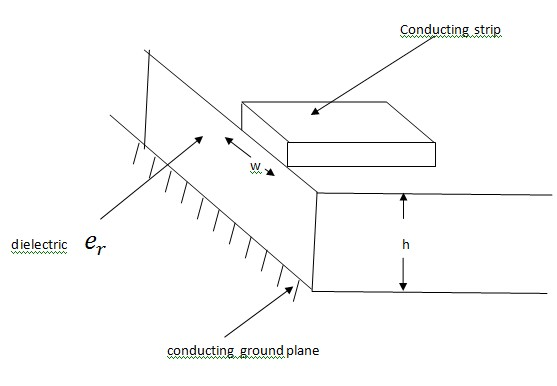
\includegraphics[width=1\linewidth]{./graphics/microstrip}
\caption{microstrip line}
\end{figure}

\begin{equation*}
Z_o=\dfrac{377}{(\sqrt{\epsilon_r}( \dfrac{W}{h})+2)}
\end{equation*}
At microwave frequency you can use a substrate like alumina for which dielectric constant is as high as 9.8.The dielectric constant value may have very wide range and $\dfrac{W}{h}$ can vary by a very wide range. So that we can realize a wide range of characteristic impedance,using high $\epsilon_r$ we can realize low $Z_o$ and high $Z_o$ with small $\epsilon_r$.
Something we can do by changing $\dfrac{W}{h}$ ratio the impedance can be varied by a large amount.When we go to high frequencies,we standardize the frequency to  $50\Omega$,if we are to connect it to a coaxial cable or make it have high impedance if we want to connect it to the parallel wire transmission line.There is a small difference however between these two connections and that is,if we take a structure which is the coaxial cable structure,with inner and outer conductor,we connect voltage to inner conductor and ground the outer conductor as shown.\\
\begin{figure}[h]
\centering
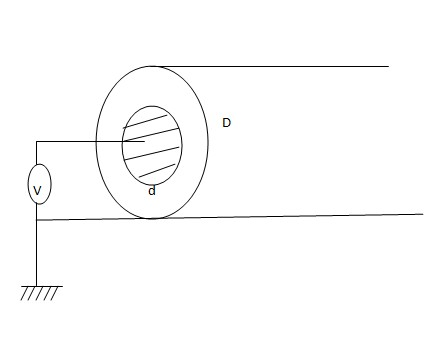
\includegraphics[width=1\linewidth]{./graphics/ground}
\caption{microstrip line}
\end{figure}
So a coaxial cable has a center conductor which voltage is connected and the outer conductor grounded.Same for the micro-strip line structure. 
We have the ground plane and the strip which carries voltage relative to the ground plane.So in both cases above the ground is defined and the voltage is applied with respect to ground. However comparing this with the parallel wire structure,this is a completely floating structure and the ground is not defined for this structure. We can either say one of these conductors is at ground or zero potential while the other is at V or we say that  there is a virtual ground in between them somewhere at the middle with one cable at $\dfrac{+V}{2}$ and the other $\dfrac{-V}{2}$ at.Hence this structure for which the ground is not defined is a floating structure while the other two have a well defined ground and the voltage is applied between the ground and the conductor.

The other two structures are called unbalanced structure and the parallel wire transmission line is called a \textbf{balanced structure}. Whenever we make connection between balanced and unbalanced lines,two things we see is that first impedance has to be matched at the junction, secondly since you are bringing now a connection between a balanced floating structure and an unbalanced structure,you require some transformer in between which can connect voltage from one bias structure to another bias structure.This device is called a \textbf{balance to unbalanced transformer or balun}.So a structure which matches the impedance as well as the nature of the cables is called BALUN (from the word Balanced Unbalanced) as shown below
\begin{figure}[h]
\centering
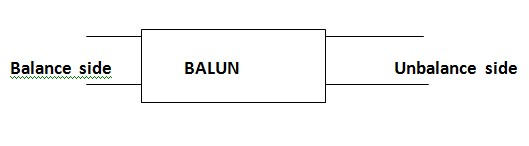
\includegraphics[width=1\linewidth]{./graphics/balun}
\caption{typical diagram of a balun}
\end{figure}
\begin{figure}[h]
\centering
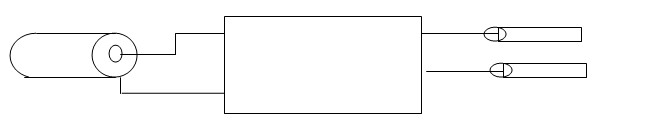
\includegraphics[width=1\linewidth]{./graphics/balun2}
\caption{typical diagram of a balun}
\end{figure}

We see this BALUN wherever we make a connection between a YAGI antenna and a TV. This is the most visible application you can see around, of course there are many other high frequency application of the BALUN. Practically when using a YAGI antenna connected to a TV,you bring in a signal from the antenna by using a flat ribbon cable to the BALUN structure which is a blackbox behind your TV set.The connector you have at the back of your TV is a coaxial connector so it is unbalanced. The impedance of the coaxial connector is 50$\Omega$, but for the flat ribbon cable coming from the antenna, it is much different compared to 50$\Omega$.So normally we introduce a small box called a BALUN and this transform the impedance from the flat  antenna ribbon cable balanced structure to the unbalanced structure.If you do not do that many times you get  the reflection from the junctions which appear in form of GHOST on the TV.So appropriate transformation of impedance on the line and also connecting balanced to unbalanced side of the network properly with the help of a BALUN,improve the quality of the reception with any high frequency signal. This essentially conclude our discussion on the transmission line 
\section{Conclusion.}
Lets recap what we have done in this very important aspect of high frequency circuit called transmission line. We saw the limitation of the analysis of the lumped circuits that is as we go to high frequency,the size of the component becomes comparable to wavelength and then the voltage and current cannot be assumed constant along any electronic component, so we introduced the concept of the distributed element.We study the transient time effect and from there we derived the relationship between voltage and current for high frequency circuits i.e for circuits over which transient time effect can't be neglected.We saw that the relationship where in form of differential equations, when we solved in form of waves, so in general at high frequencies the voltage and current exist in the form of waves in the circuits.

Then we studied the superposition of these waves and we saw that in general we got a standing wave,we also investigated under what condition you have two waves which are traveling in opposite direction or you have standing waves.So we introduced the concept of voltage reflection coefficient, which is a measure of energy reflected away  from the load.

Then we introduced the concept of MATCHING,Which means that if a load impedance is equal to the characteristics impedance,the energy is transferred from the generator to the load efficiently and there is no reflection on the line.Following this we studied impedance transformation characteristics of the  transmission lines. Then we looked at many applications of transmission line viz as circuit element,as a resonant circuit,as voltage/current stepping up transformers  and then we studied the graphical approach to analyzing  transmission line problems from the smith chart.

We also solve certain problems and towards the end of this discussion on transmission line we got expression for solving characteristics impedance for various structures which are used as transmission line at high frequencies. We saw the coaxial cable which is a very common circuit used at high frequencies.

We saw that its characteristics impedance is rather low and that it is difficult to realize high characteristics impedance using the coaxial structure. On the contrary the parallel wire structure is more capable of giving high characteristics impedances. We saw some application where the parallel and coaxial transmission line will be used,and the last was the microstrip line structure which is normally seen at microwave frequencies of few $GHz$, also when having transmission line on printed circuit board, we saw how these structure can be connected and lastly the use of a BALUN.

Today computer speeds are going into $GHz$ , \textbf{transmission line} effects is going to play a very prominent role in circuit design.Few decades back when the frequencies where not very high,electronics circuit design was quite simple, all the transmission line effect where not playing a role in the circuit. However when your chips are going to frequency of few $GHz$, your computers are going to frequency of few $GHz$,the reflections,the mismatching,all those things which we discussed become very vital in making the electronics circuit.So in today's electronic circuits, the concept of transmission line plays a very  important role.The subject of transmission line has become very important of recent years because of these high speed electronic circuits which are now part of our everyday life. 